\subsubsection{Multiple Features}
\begin{itemize}[--]
	\item A potential binary classification solution is to make the binary decision based on a threshold. eg. threshold = 0.5:
	\begin{align*}
		& h(x)\geq 0.5 & \text{predict } y = 1\\
		& h(x)< 0.5 & \text{predict }y = 0
	\end{align*}

	\item We want a classifier that results in $0\leq h\leq 1$, as we only have 2 outcomes 0, 1
\end{itemize}

\subsubsection{Hypothesis Representation}
\begin{itemize}[--]
	\item \textbf{Sigmoid/Logistic function}:
		$$g(z)=\frac{1}{1+e^{-z}}$$
	\begin{center}
		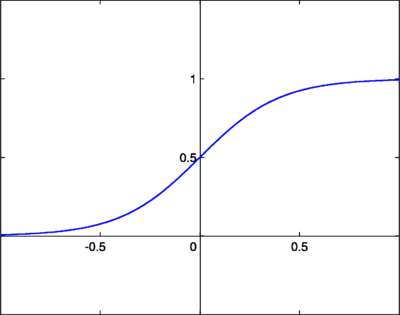
\includegraphics[scale=0.65]{sections/cs229/w3/sigmoid.png}
	\end{center}
	\item Note: there are horizontal asymptotes at 0 and 1.
	\item We will modify our original hypothesis to now be: $h(x)=g(\theta^{T}x)$, where $g$ is the previously defined sigmoid function
	\item Interpretation of hypothesis output: 
	$$h_\theta (x) = \text{ estimated probability that } y=1 \text{ on input } x$$
	\item Eg. $h(x)=0.7\to$ 70\% chance of tumor being malignant
	\item $h(x)=p(y=1|x;\theta)$ is another way of defining this.
	\item $p(y=0|x;\theta) + p(y=1|x;\theta) = 1$
\end{itemize}

\subsubsection{Decision Boundary}
\begin{itemize}[--]
	\item Suppose we predict $y=1$ if $h(x)\geq 0.5$. Graphically, we can seee that this is the same as predicting 1 when $\theta^{T}x\geq 0$
	\item \textbf{Decision Boundary}: region where $h(x)$ is equal to the threshold (the line that seperates 0 predictions vs 1 predictions).
	\item This concept can be expanded with the higher powered functions, to result in non-linear decision boundaries
	$$h(x)=g(\theta_0+\theta_1x+\theta_2 x_2 + \theta_3 x_1^2+\theta_4 x_2^2)$$
	$$\text{Predict } y=1\text{ if } -1+x_1^2+x_2^2\geq 0$$
\end{itemize}

\subsubsection{Cost Function}
\begin{itemize}[--]
	\item How do we choose/fit the parameters $\theta$?
	\item We abstract our linear regression cost function to be:
		$$j(\theta)=\frac{1}{m}\sum_{i=1}^{m}\frac{1}{2}(h(x^{(i)}-y^{(i)}))^2=\frac{1}{m}\sum_{i=1}^m\text{cost}(h(x^{(i)}, y)$$
		$$\text{cost}(h(x), y)=\frac{1}{2} (h(x)-y)^2$$

	\item However, this cost function is non-convex for logistic regression, which doesn't allow us to run gradient descent (no garuntee of global minimum reached).
	\item Let our cost function for logistic regression now be defined as:
	$$\text{cost}(h(x), y)=\begin{cases}
		-\log (h(x)) & y=1 \\
		-\log (1-h(x)) & y=0
	\end{cases}$$
	\begin{center}
		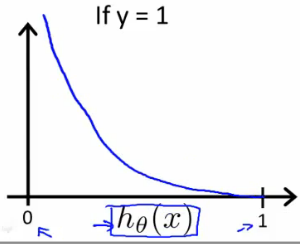
\includegraphics[scale=0.7,]{sections/cs229/w3/logisticcost.png}
		\newline
		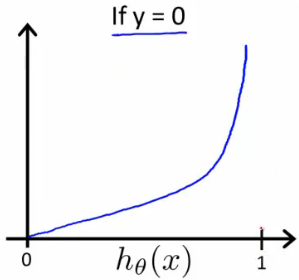
\includegraphics[scale=0.]{sections/cs229/w3/logisticcost0.png}
	\end{center}

	\item This allows us to have no cost when we were correct at our guess, but have increasingly greater cost the more wrong we were.
\end{itemize}

\subsubsection{Simplified Cost Function and Gradient Descent}
\begin{itemize}[--]
	\item We can simplify the cost function to a single formula:
	$$\text{cost}(h(x),y)=-y\log (h(x)) - (1-y) \log (1-h(x)$$
	\item This formula works because when $y=1$ the portion of the equation that is relevant for $0$ becomes $0$ via $(1-y)$
	\item Similarly for $y=0$.
	\item Note: $y\in {0, 1}$ always.
	\begin{align}
		J(\theta) &= \frac{1}{m}\sum_{i=1}^{m}\text{cost}(h(x^{(i)}), y^{(i)})
		&= -\frac{1}{m}\sum_{i=1}^{m}y^{(i)}\log h(x^{i}) + (1-y{(i)})\log (1-h(x({i})))
	\end{align}

	\item Note the negative sign was pulled out of the summation and brought in front of the summation
	\item To implement gradient descent we must first fit the parameters $\theta$ to the model by minimizing $J(\theta)$
	\item Then we can make a predition given the new $x$ using: $h(x)=\frac{1}{1+e^{-\theta^{T}x}}$
	\item We again minimize our cost function using gradient descent, where:
	$$\frac{\partial}{\partial\theta_j}J(\theta) = \frac{1}{m}\sum_{i=1}^{m} (h(x^{(i)}-y{(i)})x_j^{(i)}$$

	\item To ensure that the learning rate $\alpha$ is set properly, remember to plot the cost function ($J(\theta)$) as a function of number of iterations and make sure $J(\theta)$ is decreasing on every iteration
\end{itemize}

\subsubsection{Advanced Optimization}
\begin{itemize}[--]
	\item Optimization algorithm: has the goal of minimizing a cost function $J(\theta)$. 
	\item Given $\theta$ we have code that can compute:
	\begin{itemize}[--]
		\item $J(\theta)$ (to monitor convergence)
		\item $\frac{\partial}{\partial\theta_j}J(\theta)$ for ($j=0,1,\ldots, n$)
	\end{itemize}

	\item Gradient descent repeats the following until convergence:
	$$\theta_j := \theta_j - \alpha\frac{\partial}{\partial\theta_j}J(\theta)$$

	\item Gradient descent isn't the only optimization algorithm:
	\begin{itemize}[--]
		\item Conjugate gradient
		\item BFGS
		\item L-BFGS
	\end{itemize}

	\item They have the advantages:
	\begin{itemize}[--]
		\item No need to manually pick $\alpha$
		\item Often faster than gradient descent
	\end{itemize}

	\item And the disadvantages:
	\begin{itemize}[--]
		\item More complex
	\end{itemize}

	\item Don't implement these yourself, use package implementation
\end{itemize}

\subsubsection{Multiclass Classification: One-vs-All}
\begin{itemize}[--]
	\item Example of \textbf{multiclass classification}: email foldering/tagging: work, friends, family, hobby, etc.
	\item In \textbf{one-vs-all} we compare each classification against all other possibilities. 
	\begin{center}
		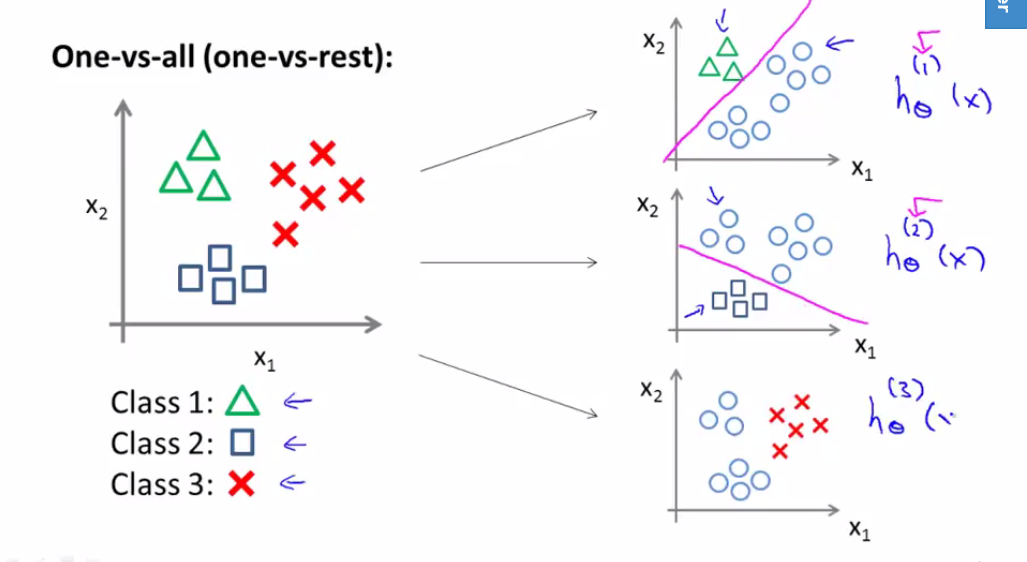
\includegraphics[scale=0.5]{sections/cs229/w3/multiclass.png}
	\end{center}

	\item This gives us a classifier for each class
	\item Each classifier estimates the probability that the value is that particular class
	\item This allows us to guess the particular class by taking the representative class of the maximum probability classifier across all classifiers
\end{itemize}